%
% Documento: Apêndices
%

\begin{apendicesenv}
\partapendices

\chapter{Tentativa de configuração do mod\_h2}
\label{apend:tentativadeconfiguracaomodh2}

Na tentativa de configurar o módulo moh\_h2 em um servidor Apache, foram usadas como referência as instruções descritas no site do projeto\footnote{https://github.com/icing/mod\_h2} no mês de Agosto de 2015. Mas apesar das instruções estarem bem explicadas, o final do processo de configuração ficou um pouco confuso e com isso não foi possível concluir a instalação do mod\_h2 com sucesso.

Abaixo encontra-se o passo-a-passo realizado.

\begin{enumerate}
	\item Clone o projeto para conseguir o código: \textit{git clone https://github.com/icing/mod\_h2.git}
	\item Instale as dependências de sistema necessárias: \textit{sudo apt-get install git gcc g++ libpcre3-dev libcunit1-dev libev-dev libjansson-dev libjemalloc-dev cython make binutils autoconf automake autotools-dev libtool pkg-config zlib1g-dev libssl-dev libxml2-dev libevent-dev python3.4-dev libevent-openssl-2.0-5 php5-cgi python-setuptools}
	\item Entre na pasta do projeto: \textit{cd mod\_h2-x.x.x}
	\item Gere os arquivos necessários para o automake e o autoconf funcionarem: \textit{autoreconf -i}
	\item Gere o arquivo de compilação: \textit{automake}
	\item Gere o arquivo de configuração: \textit{autoconf}
	\item Execute o \textit{script} de configuração: \textit{./configure --enable-sandbox}\footnote{A instalação utilizando a \textit{sandbox} garante que todas as dependências para configurar o servidor serão instaladas.}
	\item Compile o código: \textit{make}
	\item Encontre o arquivo binário (mod\_h2.so) gerado
	\item Crie ma pasta chamada \textit{modules} e copie o arquivo binário para ela
	\item Mude a configuração geral do servidor Apache para utilizar o novo módulo:
		\begin{center}
			\textit{sudo nano apache2.conf}
			Adicione o seguinte código na última linha do arquivo: \textit{LoadModule h2\_module /etc/apache2/modules/mod\_h2.so} (onde /etc/apache2/modules/mod\_h2.so é o caminho para seu arquivo binário)
		\end{center}
	\item Reinicie o servidor: \textit{sudo service apache2 restart}
\end{enumerate}

Juntamente com as configurações de navegador necessárias para garantir que as requisições serão feitas utilizando o novo protocolo, essa sequencia de passos deveria ser o suficiente para garantir que o servidor Apache iria utilizar o protocolo HTTP/2. Mas apesar de nenhum erro ter ocorrido durante o processo, a comunicação dos dado não passou a ser realizada com o HTTP/2.

Como o mod\_h2 é um projeto que está em desenvolvimento, muitas atualizações são feitas toda semana e a documentação sempre está evoluindo. Sendo assim pode se esperar que a documentação esteja mais completa na data de publicação deste trabalho e que a configuração do módulo seja mais fácil.

Ademais, vale ressaltar que o mod\_h2 foi doado à Apache Foundation e que ele se tornará o módulo oficial para o HTTP/2 do servidor Apache na sua versão 2.4. O lançamento da nova versão do servidor está prevista para Outubro de 2015.

\chapter{Configurando \textit{nghttp2}}
\label{apend:configurandonghttp2}

Apesar de descrita no site oficial do projeto\footnote{https://github.com/tatsuhiro-t/nghttp2}, a configuração do \textit{nghttp2} só foi possível graças a \citeonline{nghttp2config}. Em seu artigo Tollman descreve bem detalhadamente o processo de instalação do \textit{nghttp2} e suas dependências. Enquanto que no site oficial do projeto a instalação das dependências fica a cargo do desenvolvedor. 

Abaixo encontra-se um resumo dos passos descritos por Tollman.

\subsection{Instalando dependências}
Instale todas as dependências básicas:
	\begin{center}
		\textit{sudo apt-get install make binutils autoconf automake autotools-dev libtool pkg-config zlib1g-dev libcunit1-dev libssl-dev libxml2-dev libev-dev libevent-dev libjansson-dev libjemalloc-dev python3.4-dev g++ g++-mingw-w64-i686 git python3-setuptools}	
		\textit{sudo easy\_install3 pip}
		\textit{sudo pip3.4 install -U cython}
	\end{center}

Instale o Spdylay, que serve como base para o \textit{nghttp2}
\begin{enumerate}
	\item Crie uma pasta para o código compilado: \textit{mkdir ~/src}
	\item Clone o projeto: \textit{git clone https://github.com/tatsuhiro-t/spdylay.git ~/src/spdylay}
	\item Entre na pasta: \textit{cd ~/src/spdylay}
	\item Gere os arquivos necessários para o automake e o autoconf funcionarem: \textit{autoreconf -i}
	\item Gere o arquivo de compilação: \textit{automake}
	\item Gere o arquivo de configuração: \textit{autoconf}
	\item Execute o \textit{script} de configuração: \textit{./configure}
	\item Compile o código: \textit{make}
	\item Execute o arquivo compilado: \textit{sudo make install}
	\item Atualize o seu sistema: \textit{sudo updatedb}
	\item Localize a biblioteca spylay: \textit{locate libspdylay.so.7}
	\item Configure os links de execução da biblioteca:
		\begin{center}
			\textit{sudo ln -s /usr/local/lib/libspdylay.so.7 /lib/x86\_64-linux-gnu/libspdylay.so.7}
			\textit{sudo ln -s /usr/local/lib/libspdylay.so.7.2.0 /lib/x86\_64-linux-gnu/libspdylay.so.7.2.0}
			\textit{sudo ldconfig}
		\end{center}
\end{enumerate}

Seguindo esses passos todas dependências necessárias para a instalação do \textit{nghttps} estão prontas para serem usadas.

\subsection{Instalando a aplicação}
O processo de instalação do \textit{nghttp2} é mais uma vez um processo de compilação do código fonte e configuração da biblioteca.

\begin{enumerate}
	\item Clone o projeto: \textit{git clone https://github.com/tatsuhiro-t/nghttp2.git ~/src/nghttp2}
	\item Entre na pasta: \textit{cd ~/src/nghttp2}
	\item Gere os arquivos necessários para o automake e o autoconf funcionarem: \textit{autoreconf -i}
	\item Gere o arquivo de compilação: \textit{automake}
	\item Gere o arquivo de configuração: \textit{autoconf}
	\item Execute o \textit{script} de configuração: \textit{./configure PYTHON=/usr/bin/python3} (confirmar o uso do \textit{python3} é muito importante, pois por padrão o \textit{python2} que costuma ser utilizado)
	\item Compile o código: \textit{make}
	\item Execute o arquivo compilado: \textit{sudo make install}
	\item Atualize o seu sistema: \textit{sudo updatedb}
	\item Localize a biblioteca spylay: \textit{locate libnghttp2.so.14}
	\item Configure os links de execução da biblioteca:
		\begin{center}
			\textit{sudo ln -s /usr/local/lib/libnghttp2.so.14 /lib/x86\_64-linux-gnu/libnghttp2.so.14}
			\textit{sudo ln -s /usr/local/lib/libnghttp2.so.14.0.2 /lib/x86\_64-linux-gnu/libnghttp2.so.14.0.2}
			\textit{sudo ldconfig}
		\end{center}
\end{enumerate}

Vale ressaltar que as versões especificadas nos arquivos gerados dependem das versões dos códigos que estão sendo utilizados.

\lstset{
	frame=single,
    breaklines=true,
    language=HTML
    }
\chapter{Faça menos requisições HTTP: Arquivos Separados}
\label{apend:codigo_facamenosrequisicoeshttp_sep}

\begin{lstlisting}
<!DOCTYPE html>
<html>
<head>
<link rel="stylesheet" href="css/animate.css">
<link rel="stylesheet" href="css/bootstrap.min.css">
<link rel="stylesheet" href="css/bootstrap-theme.min.css">
<link rel="stylesheet" href="css/font-awesome.min.css">
<link rel="stylesheet" href="css/fullcalendar.min.css">
<link rel="stylesheet" href="css/normalize.css">
<link rel="stylesheet" href="css/skeleton.css">
	
<link rel="stylesheet" href="css/animate - Copy.css">
<link rel="stylesheet" href="css/bootstrap.min - Copy.css">
<link rel="stylesheet" href="css/bootstrap-theme.min - Copy.css">
<link rel="stylesheet" href="css/font-awesome.min - Copy.css">
<link rel="stylesheet" href="css/fullcalendar.min - Copy.css">
<link rel="stylesheet" href="css/normalize - Copy.css">
<link rel="stylesheet" href="css/skeleton - Copy.css">
</head>

<body>

<h1>My First Heading</h1>

<p>My first paragraph.</p>

<img src="imgs/1.jpg" />
<img src="imgs/2.jpg" />
<img src="imgs/3.jpg" />
<img src="imgs/4.jpg" />
<img src="imgs/5.jpg" />
<img src="imgs/6.jpg" />
<img src="imgs/7.jpg" />
<img src="imgs/8.jpg" />
<img src="imgs/9.jpg" />
<img src="imgs/10.jpg" />
<img src="imgs/11.jpg" />
<img src="imgs/12.jpg" />
<img src="imgs/13.jpg" />
<img src="imgs/14.png" />
<img src="imgs/15.png" />
<img src="imgs/16.jpg" />
<img src="imgs/17.jpg" />
<img src="imgs/18.jpg" />
<img src="imgs/19.jpg" />
<img src="imgs/20.jpg" />
<img src="imgs/21.jpg" />
<img src="imgs/22.jpg" />
<img src="imgs/23.jpg" />
<img src="imgs/24.jpg" />
<img src="imgs/25.jpg" />
<img src="imgs/26.jpg" />
<img src="imgs/27.jpg" />
<img src="imgs/28.jpg" />
	

<script src="js/jquery-2.1.4.min.js"></script>
<script src="js/angular.min.js"></script>
<script src="js/backbone.js"></script>
<script src="js/bootstrap.min.js"></script>
<script src="js/d3.min.js"></script>
<script src="js/ember-data.min.js"></script>
<script src="js/fullcalendar.min.js"></script>
<script src="js/highcharts.js"></script>
<script src="js/moment-with-locales.min.js"></script>
<script src="js/require.js"></script>
</body>
</html>
\end{lstlisting}

\chapter{Faça menos requisições HTTP: Arquivos Concatenados}
\label{apend:codigo_facamenosrequisicoeshttp_concat}

\begin{lstlisting}
<!DOCTYPE html>
<html>
<head>
<link rel="stylesheet" href="css/minified.css">
</head>

<body>

<h1>My First Heading</h1>
<p>My first paragraph.</p>
	
<img src="imgs/1.jpg" />
<img src="imgs/2.jpg" />
<img src="imgs/3.jpg" />
<img src="imgs/4.jpg" />
<img src="imgs/5.jpg" />
<img src="imgs/6.jpg" />
<img src="imgs/7.jpg" />
<img src="imgs/8.jpg" />
<img src="imgs/9.jpg" />
<img src="imgs/10.jpg" />
<img src="imgs/11.jpg" />
<img src="imgs/12.jpg" />
<img src="imgs/13.jpg" />
<img src="imgs/14.png" />
<img src="imgs/15.png" />
<img src="imgs/16.jpg" />
<img src="imgs/17.jpg" />
<img src="imgs/18.jpg" />
<img src="imgs/19.jpg" />
<img src="imgs/20.jpg" />
<img src="imgs/21.jpg" />
<img src="imgs/22.jpg" />
<img src="imgs/23.jpg" />
<img src="imgs/24.jpg" />
<img src="imgs/25.jpg" />
<img src="imgs/26.jpg" />
<img src="imgs/27.jpg" />
<img src="imgs/28.jpg" />

	<script src="js/minified.js"></script>
</body>
</html>

\end{lstlisting}

\chapter{Reduza o número de pesquisas DNS: Multiplas CDN}
\label{apend:codigo_reduzaonumerodepesquisasdns_mult}	

\begin{lstlisting}
<!DOCTYPE html>
<html>
<head>
<link rel="stylesheet" href="//cdnjs.cloudflare.com/ajax/libs/animate.css/3.4.0/animate.min.css">
<link rel="stylesheet" href="//maxcdn.bootstrapcdn.com/bootstrap/3.3.5/css/bootstrap.min.css">
<link rel="stylesheet" href="//maxcdn.bootstrapcdn.com/font-awesome/4.4.0/css/font-awesome.min.css">	
<link rel="stylesheet" href="//cdnjs.cloudflare.com/ajax/libs/fullcalendar/2.0.2/fullcalendar.js">
<link rel="stylesheet" href="//cdn.bootcss.com/skeleton/2.0.4/skeleton.css">
<link rel="stylesheet" href="css/normalize.css">
</head>

<body>

<h1>My First Heading</h1>
<p>My first paragraph.</p>

<img src="imgs/1.jpg" />
<img src="imgs/2.jpg" />
<img src="imgs/3.jpg" />
<img src="imgs/4.jpg" />
<img src="imgs/5.jpg" />
<img src="imgs/6.jpg" />
<img src="imgs/7.jpg" />
<img src="imgs/8.jpg" />
<img src="imgs/9.jpg" />
<img src="imgs/10.jpg" />
<img src="imgs/11.jpg" />
<img src="imgs/12.jpg" />
<img src="imgs/13.jpg" />
<img src="imgs/14.png" />
<img src="imgs/15.png" />
<img src="imgs/16.jpg" />
<img src="imgs/17.jpg" />
<img src="imgs/18.jpg" />
<img src="imgs/19.jpg" />
<img src="imgs/20.jpg" />
<img src="imgs/21.jpg" />
<img src="imgs/22.jpg" />
<img src="imgs/23.jpg" />
<img src="imgs/24.jpg" />
<img src="imgs/25.jpg" />
<img src="imgs/26.jpg" />
<img src="imgs/27.jpg" />
<img src="imgs/28.jpg" />

<script src="//ajax.googleapis.com/ajax/libs/jquery/2.1.4/jquery.min.js"></script>
<script src="//maxcdn.bootstrapcdn.com/bootstrap/3.3.5/js/bootstrap.min.js"></script>
<script src="//ajax.googleapis.com/ajax/libs/angularjs/1.3.14/angular.min.js"></script>
<script src="//cdnjs.cloudflare.com/ajax/libs/d3/3.5.6/d3.js"></script>
<script src="//cdn.bootcss.com/ember.js/2.1.0-beta.2/ember.js"></script>
<script src="js/require.js"></script>	
</body>
</html>

\end{lstlisting}

\chapter{Reduza o número de pesquisas DNS: Única CDN}
\label{apend:codigo_reduzaonumerodepesquisasdns_unic}	

\begin{lstlisting}
<!DOCTYPE html>
<html>
<head>
<link rel="stylesheet" href="//cdnjs.cloudflare.com/ajax/libs/animate.css/3.4.0/animate.min.css">
<link rel="stylesheet" href="//cdnjs.cloudflare.com/ajax/libs/twitter-bootstrap/4.0.0-alpha/js/bootstrap.min.js">
<link rel="stylesheet" href="//cdnjs.cloudflare.com/ajax/libs/font-awesome/4.4.0/css/font-awesome.min.css">	
<link rel="stylesheet" href="//cdnjs.cloudflare.com/ajax/libs/fullcalendar/2.0.2/fullcalendar.js">
<link rel="stylesheet" href="//cdnjs.cloudflare.com/ajax/libs/skeleton/2.0.4/skeleton.css">
<link rel="stylesheet" href="//cdnjs.cloudflare.com/ajax/libs/normalize/3.0.3/normalize.css">
</head>

<body>

<h1>My First Heading</h1>
<p>My first paragraph.</p>

<img src="imgs/1.jpg" />
<img src="imgs/2.jpg" />
<img src="imgs/3.jpg" />
<img src="imgs/4.jpg" />
<img src="imgs/5.jpg" />
<img src="imgs/6.jpg" />
<img src="imgs/7.jpg" />
<img src="imgs/8.jpg" />
<img src="imgs/9.jpg" />
<img src="imgs/10.jpg" />
<img src="imgs/11.jpg" />
<img src="imgs/12.jpg" />
<img src="imgs/13.jpg" />
<img src="imgs/14.png" />
<img src="imgs/15.png" />
<img src="imgs/16.jpg" />
<img src="imgs/17.jpg" />
<img src="imgs/18.jpg" />
<img src="imgs/19.jpg" />
<img src="imgs/20.jpg" />
<img src="imgs/21.jpg" />
<img src="imgs/22.jpg" />
<img src="imgs/23.jpg" />
<img src="imgs/24.jpg" />
<img src="imgs/25.jpg" />
<img src="imgs/26.jpg" />
<img src="imgs/27.jpg" />
<img src="imgs/28.jpg" />

<script src="//cdnjs.cloudflare.com/ajax/libs/jquery/2.1.4/jquery.min.js"></script>
<script src="//cdnjs.cloudflare.com/ajax/libs/twitter-bootstrap/3.3.5/js/bootstrap.min.js"></script>
<script src="//cdnjs.cloudflare.com/ajax/libs/angular.js/1.3.14/angular.min.js"></script>
<script src="//cdnjs.cloudflare.com/ajax/libs/d3/3.5.6/d3.js"></script>
<script src="//cdnjs.cloudflare.com/ajax/libs/ember.js/2.1.0-beta.2/ember.js"></script>
<script src="//cdnjs.cloudflare.com/ajax/libs/require.js/2.1.20/require.min.js"></script>	
</body>
</html>

\end{lstlisting}

\chapter{Quebrando domínios dominantes}
\label{apend:quebrandodominiodominantes}

Para duas CDNs
\begin{lstlisting}
<!DOCTYPE html>
<html>
<head>
<link rel="stylesheet" href="//cdnjs.cloudflare.com/ajax/libs/animate.css/3.4.0/animate.min.css">
<link rel="stylesheet" href="//maxcdn.bootstrapcdn.com/bootstrap/3.3.5/css/bootstrap.min.css">
<link rel="stylesheet" href="//maxcdn.bootstrapcdn.com/font-awesome/4.4.0/css/font-awesome.min.css">	
<link rel="stylesheet" href="//cdnjs.cloudflare.com/ajax/libs/fullcalendar/2.0.2/fullcalendar.js">
<link rel="stylesheet" href="//cdnjs.cloudflare.com/ajax/libs/skeleton/2.0.4/skeleton.css">
<link rel="stylesheet" href="//cdnjs.cloudflare.com/ajax/libs/normalize/3.0.2/normalize.css">
</head>

<body>

<h1>My First Heading</h1>
<p>My first paragraph.</p>
	
<img src="imgs/1.jpg" />
<img src="imgs/2.jpg" />
<img src="imgs/3.jpg" />
<img src="imgs/4.jpg" />
<img src="imgs/5.jpg" />
<img src="imgs/6.jpg" />
<img src="imgs/7.jpg" />
<img src="imgs/8.jpg" />
<img src="imgs/9.jpg" />
<img src="imgs/10.jpg" />
<img src="imgs/11.jpg" />
<img src="imgs/12.jpg" />
<img src="imgs/13.jpg" />
<img src="imgs/14.png" />
<img src="imgs/15.png" />
<img src="imgs/16.jpg" />
<img src="imgs/17.jpg" />
<img src="imgs/18.jpg" />
<img src="imgs/19.jpg" />
<img src="imgs/20.jpg" />
<img src="imgs/21.jpg" />
<img src="imgs/22.jpg" />
<img src="imgs/23.jpg" />
<img src="imgs/24.jpg" />
<img src="imgs/25.jpg" />
<img src="imgs/26.jpg" />
<img src="imgs/27.jpg" />
<img src="imgs/28.jpg" />

<script src="//cdnjs.cloudflare.com/ajax/libs/jquery/2.1.4/jquery.min.js"></script>
<script src="//maxcdn.bootstrapcdn.com/bootstrap/3.3.5/js/bootstrap.min.js"></script>
<script src="//cdnjs.cloudflare.com/ajax/libs/angular.js/1.3.14/angular.min.js"></script>
<script src="//cdnjs.cloudflare.com/ajax/libs/d3/3.5.6/d3.js"></script>
<script src="//cdnjs.cloudflare.com/ajax/libs/ember.js/2.1.0-beta.2/ember.js"></script>
<script src="//cdnjs.cloudflare.com/ajax/libs/require.js/2.1.20/require.min.js"></script>	
</body>
</html>
\end{lstlisting}

Para três CDNs
\begin{lstlisting}
<!DOCTYPE html>
<html>
<head>
<link rel="stylesheet" href="//cdnjs.cloudflare.com/ajax/libs/animate.css/3.4.0/animate.min.css">
<link rel="stylesheet" href="//maxcdn.bootstrapcdn.com/bootstrap/3.3.5/css/bootstrap.min.css">
<link rel="stylesheet" href="//maxcdn.bootstrapcdn.com/font-awesome/4.4.0/css/font-awesome.min.css">	
<link rel="stylesheet" href="//cdnjs.cloudflare.com/ajax/libs/fullcalendar/2.0.2/fullcalendar.js">
<link rel="stylesheet" href="//cdn.bootcss.com/skeleton/2.0.4/skeleton.css">
<link rel="stylesheet" href="//cdnjs.cloudflare.com/ajax/libs/normalize/3.0.2/normalize.css">
</head>

<body>

<h1>My First Heading</h1>
<p>My first paragraph.</p>
	
<img src="imgs/1.jpg" />
<img src="imgs/2.jpg" />
<img src="imgs/3.jpg" />
<img src="imgs/4.jpg" />
<img src="imgs/5.jpg" />
<img src="imgs/6.jpg" />
<img src="imgs/7.jpg" />
<img src="imgs/8.jpg" />
<img src="imgs/9.jpg" />
<img src="imgs/10.jpg" />
<img src="imgs/11.jpg" />
<img src="imgs/12.jpg" />
<img src="imgs/13.jpg" />
<img src="imgs/14.png" />
<img src="imgs/15.png" />
<img src="imgs/16.jpg" />
<img src="imgs/17.jpg" />
<img src="imgs/18.jpg" />
<img src="imgs/19.jpg" />
<img src="imgs/20.jpg" />
<img src="imgs/21.jpg" />
<img src="imgs/22.jpg" />
<img src="imgs/23.jpg" />
<img src="imgs/24.jpg" />
<img src="imgs/25.jpg" />
<img src="imgs/26.jpg" />
<img src="imgs/27.jpg" />
<img src="imgs/28.jpg" />

<script src="//cdn.bootcss.com/jquery/2.1.4/jquery.min.js"></script>
<script src="//maxcdn.bootstrapcdn.com/bootstrap/3.3.5/js/bootstrap.min.js"></script>
<script src="//cdn.bootcss.com/angular.js/1.3.4/angular.min.js"></script>
<script src="//cdnjs.cloudflare.com/ajax/libs/d3/3.5.6/d3.js"></script>
<script src="//cdn.bootcss.com/ember.js/2.1.0-beta.2/ember.js"></script>
<script src="//cdn.bootcss.com/require.js/2.1.20/require.min.js"></script>	
</body>
</html>

\end{lstlisting}

\end{apendicesenv}

\chapter{Gráficos em cascata}
\label{apend:graficosemcascata}

\begin{figure}[!htb]
    \centering
    \caption{Cascata "Reduza requisições HTTP" - Arquivos separados - HTTP/1.1.}
    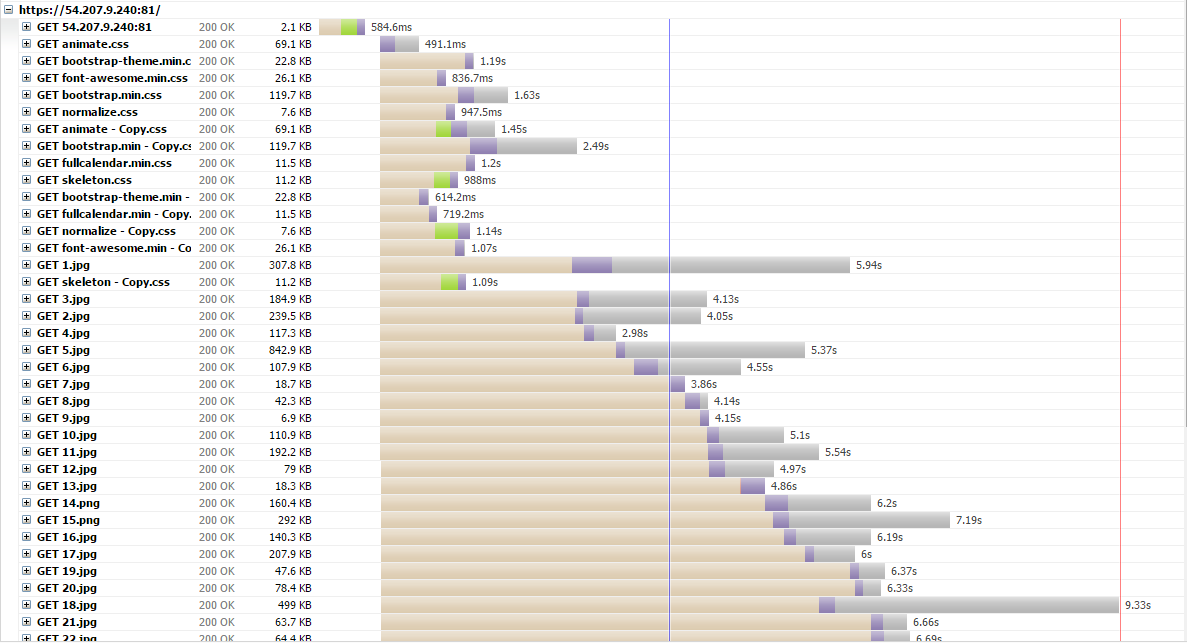
\includegraphics[width=1.0\textwidth]{./04-figuras/cascatas/separados_http11}
\end{figure}

\begin{figure}[!htb]
    \centering
    \caption{Cascata "Faça menos requisições HTTP" - Arquivos separados - HTTP/2.}
    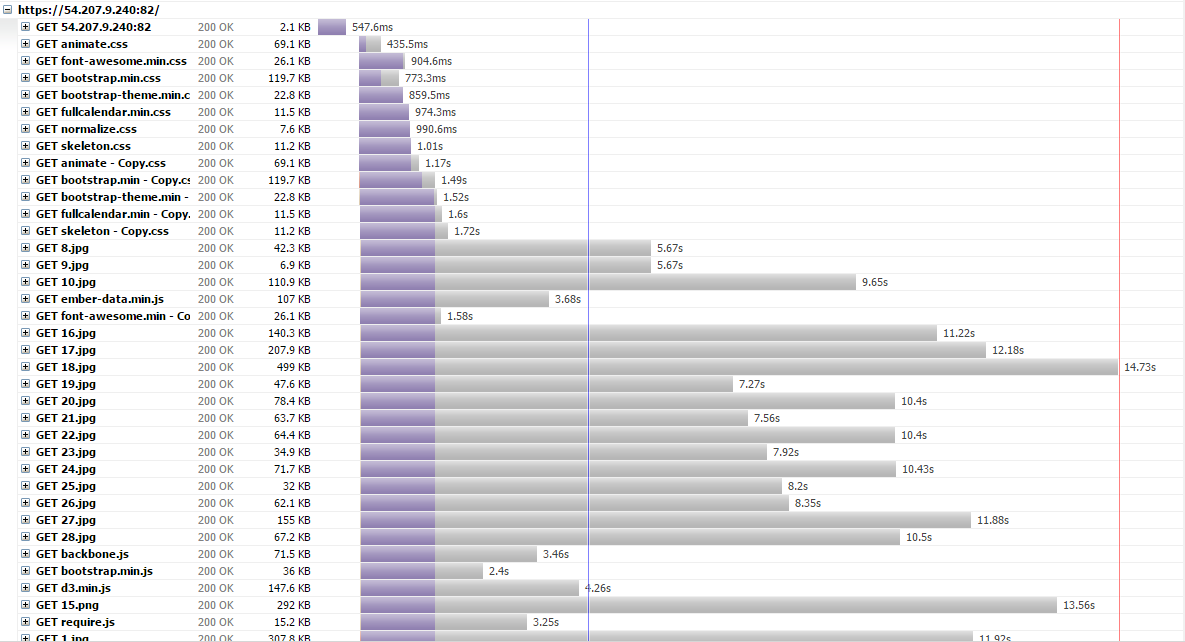
\includegraphics[width=1.0\textwidth]{./04-figuras/cascatas/separados_http2}
\end{figure}

\begin{figure}[!htb]
    \centering
    \caption{Cascata "Faça menos requisições HTTP" - Arquivos concatenados - HTTP/1.1.}
    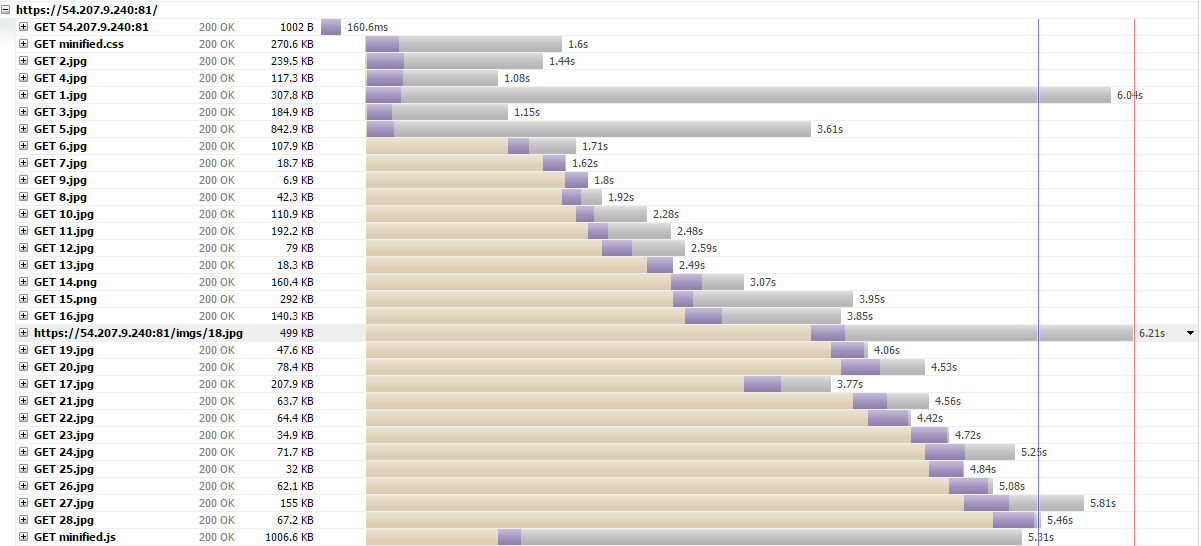
\includegraphics[width=1.0\textwidth]{./04-figuras/cascatas/concatenado_http11}
\end{figure}

\begin{figure}[!htb]
    \centering
    \caption{Cascata "Faça menos requisições HTTP" - Arquivos concatenados - HTTP/2.}
    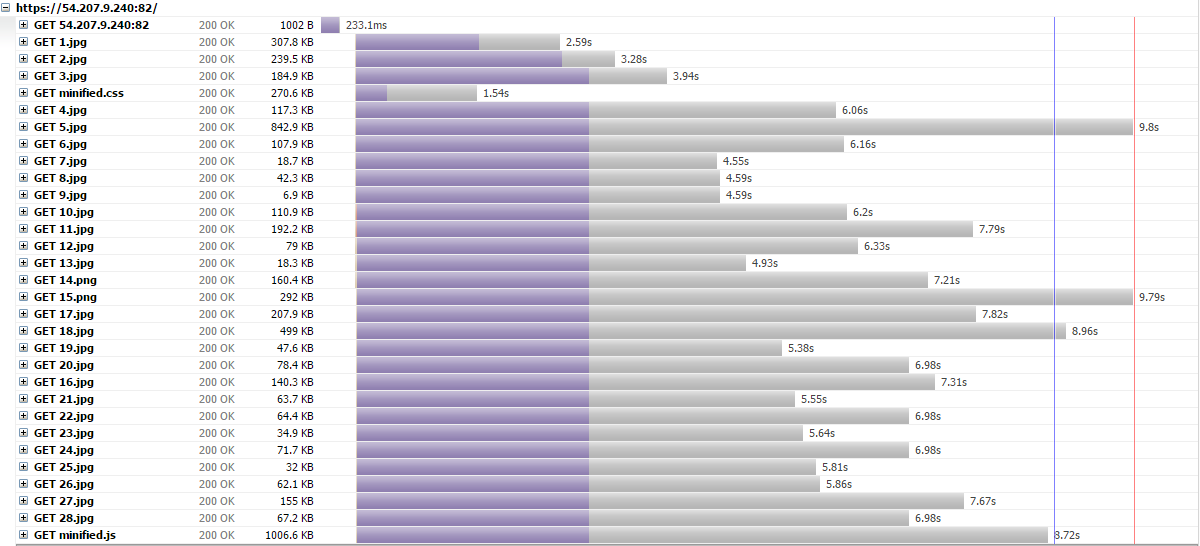
\includegraphics[width=1.0\textwidth]{./04-figuras/cascatas/concatenado_http2}
\end{figure}

\begin{figure}[!htb]
    \centering
    \caption{Cascata "Reduza o número de pesquisas DNS" - Única CDN - HTTP/1.1.}
    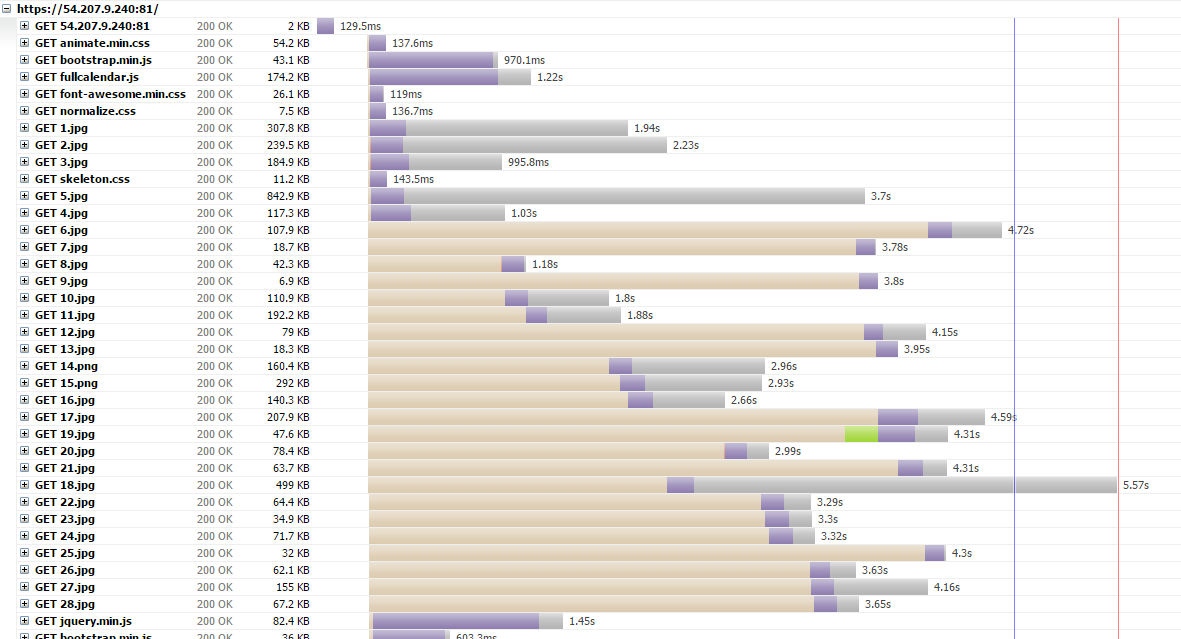
\includegraphics[width=1.0\textwidth]{./04-figuras/cascatas/single_http11}
\end{figure}

\begin{figure}[!htb]
    \centering
    \caption{Cascata "Reduza o número de pesquisas DNS" - Única CDN - HTTP/2.}
    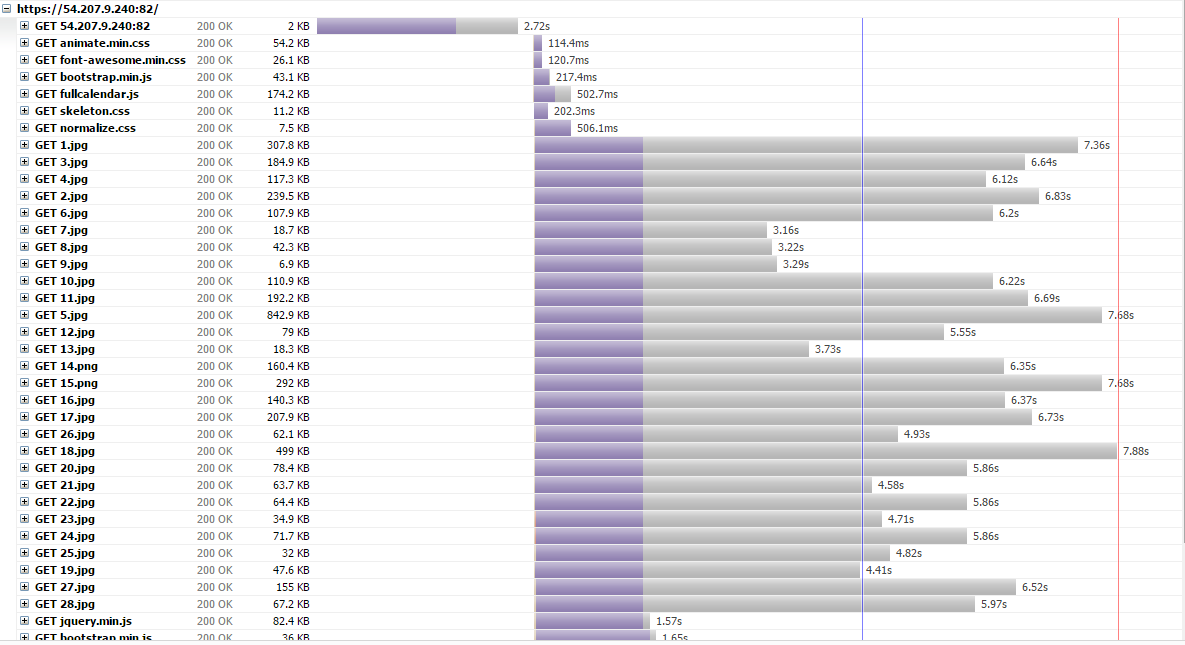
\includegraphics[width=1.0\textwidth]{./04-figuras/cascatas/single_http2}
\end{figure}

\begin{figure}[!htb]
    \centering
    \caption{Cascata "Reduza o número de pesquisas DNS" - Multiplas CDN - HTTP/1.1.}
    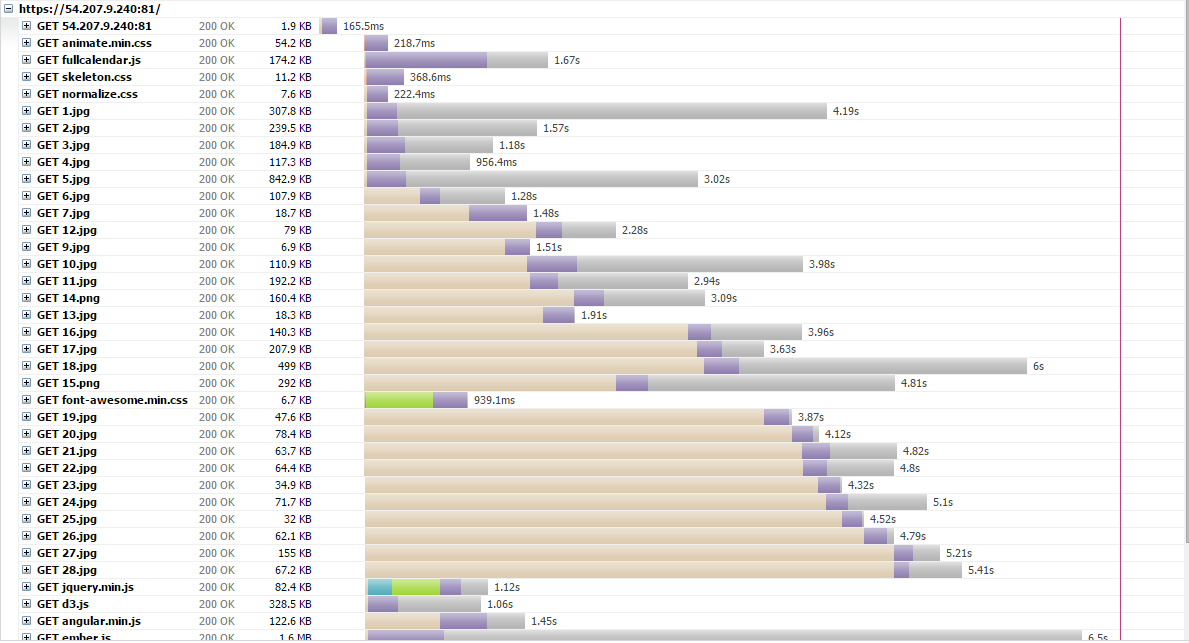
\includegraphics[width=1.0\textwidth]{./04-figuras/cascatas/multiple_http11}
\end{figure}

\begin{figure}[!htb]
    \centering
    \caption{Cascata "Reduza o número de pesquisas DNS" - Multiplas CDNs - HTTP/2.}
    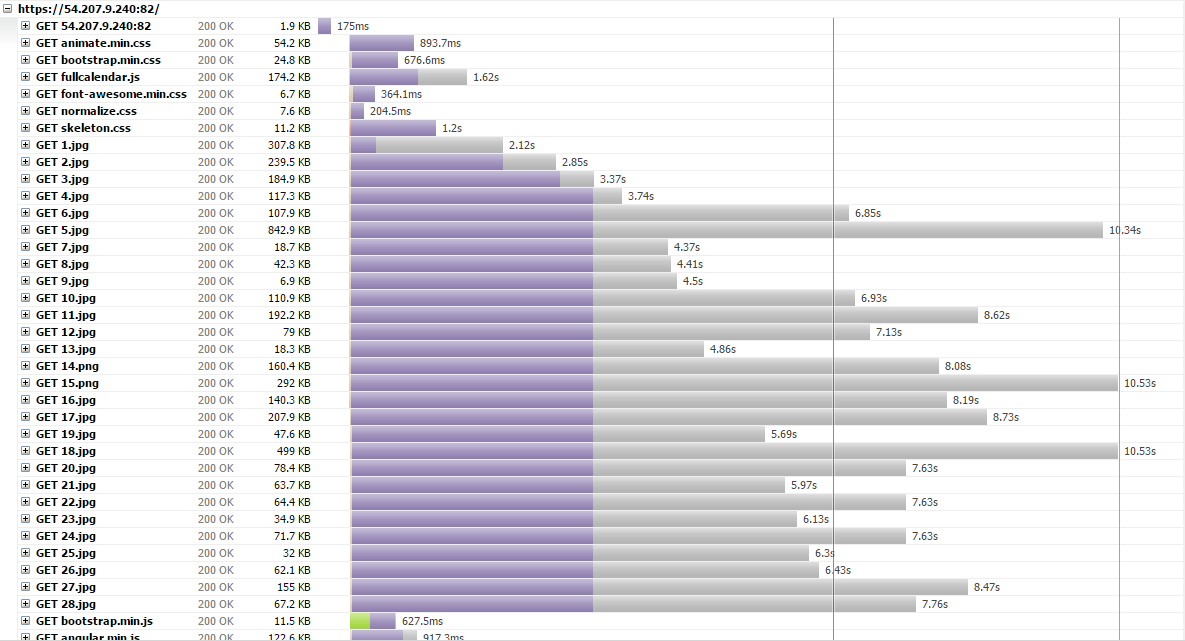
\includegraphics[width=1.0\textwidth]{./04-figuras/cascatas/multiple_http2}
\end{figure}

\begin{figure}[!htb]
    \centering
    \caption{Cascata "Quebrando domínios dominantes" - 2 CDNs - HTTP/1.1.}
    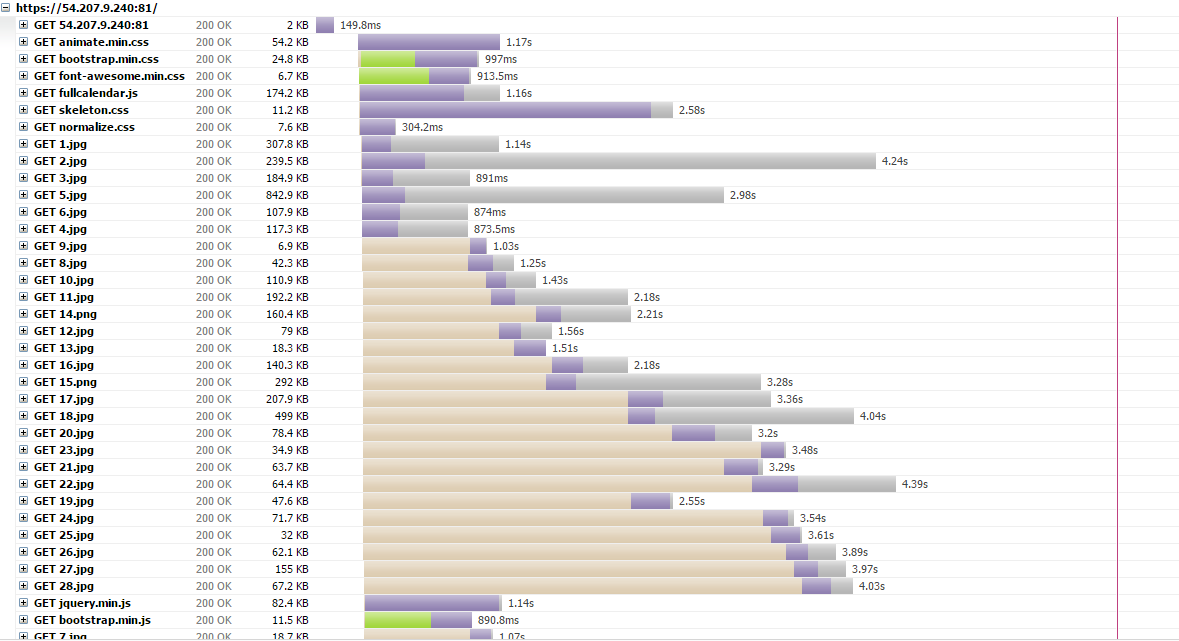
\includegraphics[width=1.0\textwidth]{./04-figuras/cascatas/2cds_http11}
\end{figure}

\begin{figure}[!htb]
    \centering
    \caption{Cascata "Quebrando domínios dominantes" - 2 CDNs - HTTP/2.}
    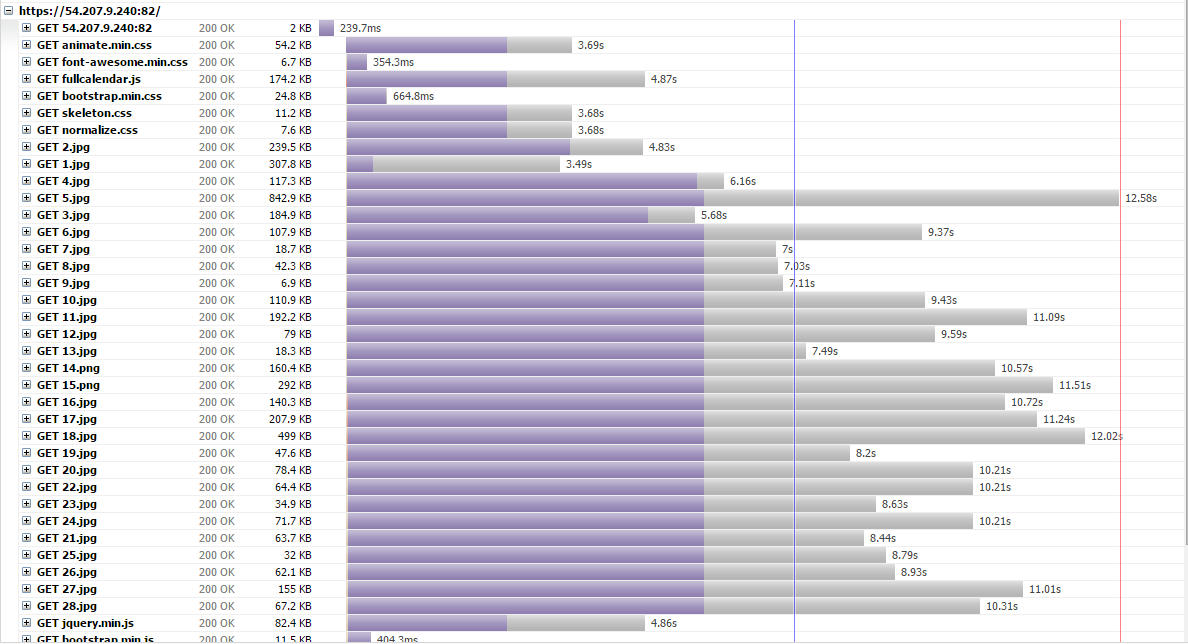
\includegraphics[width=1.0\textwidth]{./04-figuras/cascatas/2cds_http2}
\end{figure}

\begin{figure}[!htb]
    \centering
    \caption{Cascata "Quebrando domínios dominantes" - 3 CDNs - HTTP/1.1.}
    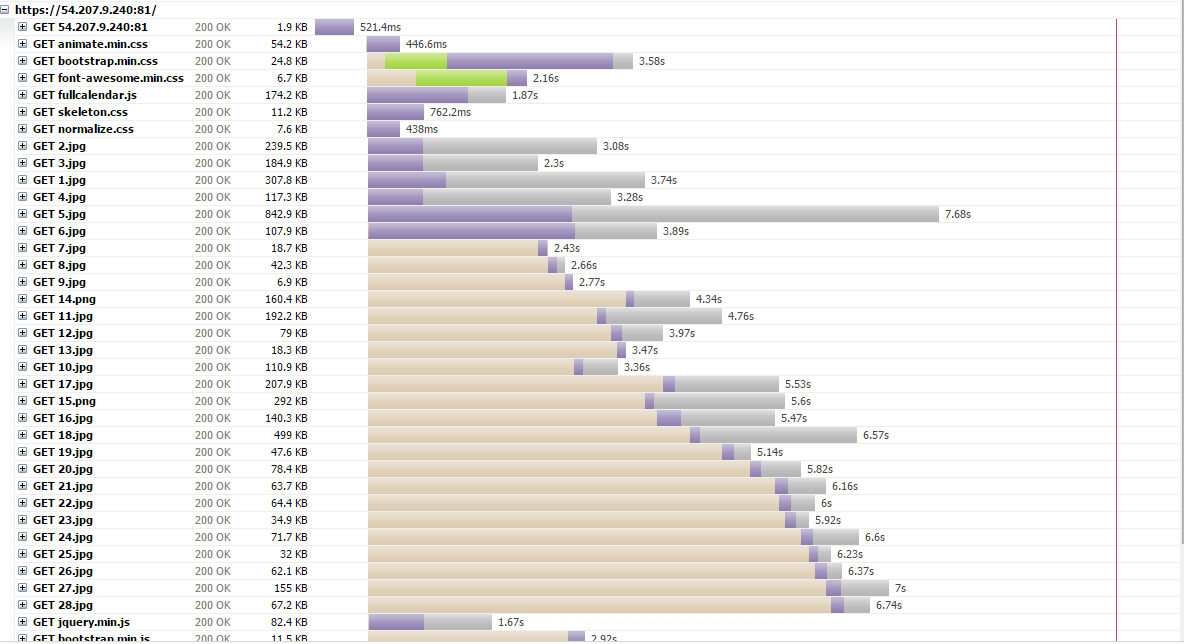
\includegraphics[width=1.0\textwidth]{./04-figuras/cascatas/3cds_http11}
\end{figure}

\begin{figure}[!htb]
    \centering
    \caption{Cascata "Quebrando domínios dominantes" - 3 CDNs - HTTP/2.}
    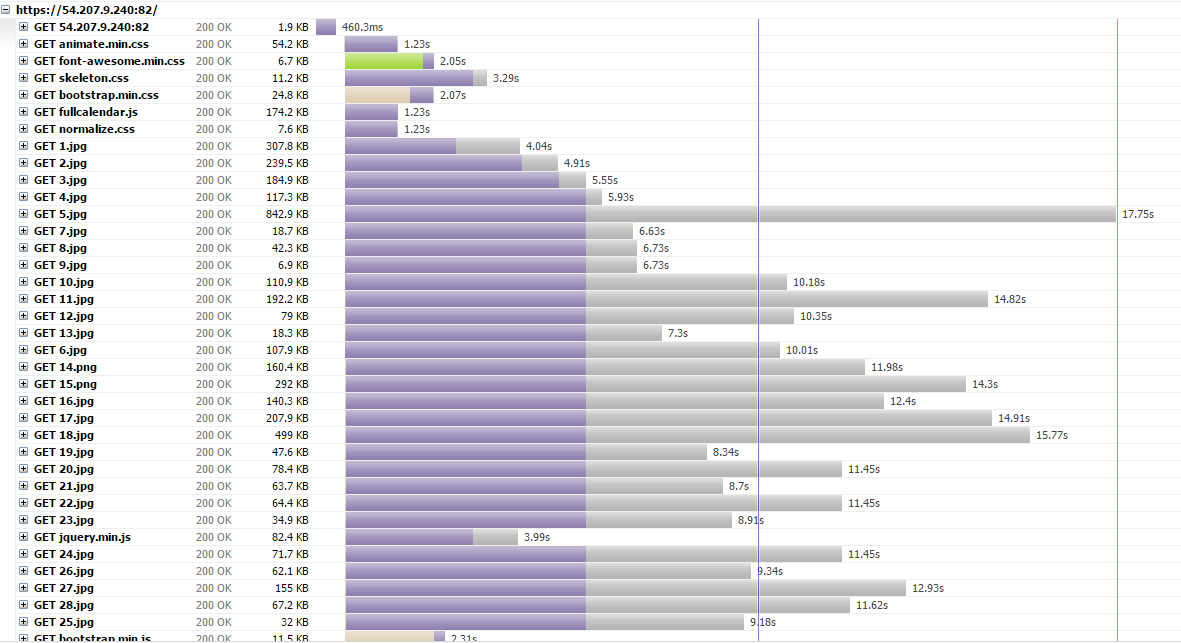
\includegraphics[width=1.0\textwidth]{./04-figuras/cascatas/3cds_http2}
\end{figure}

\begin{figure}[!htb]
    \centering
    \caption{Cascata "Template" - HTTP/1.1.}
    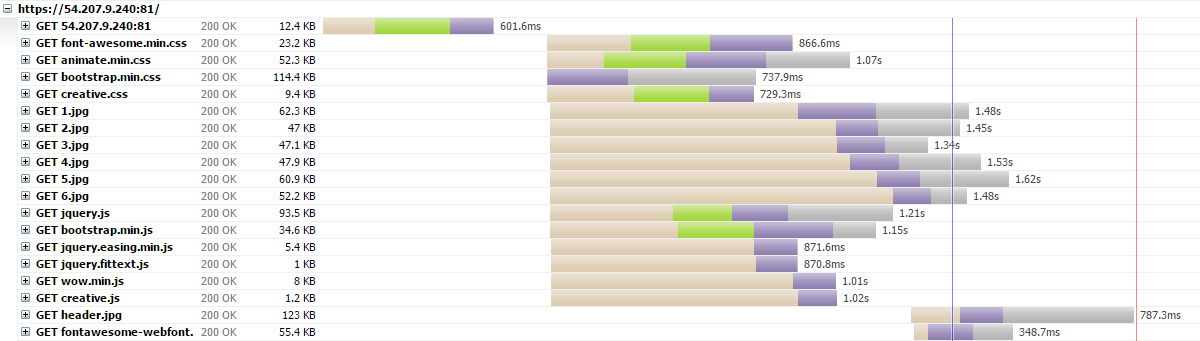
\includegraphics[width=1.0\textwidth]{./04-figuras/cascatas/template_http11}
\end{figure}

\begin{figure}[!htb]
    \centering
    \caption{Cascata "Template" - HTTP/2.}
    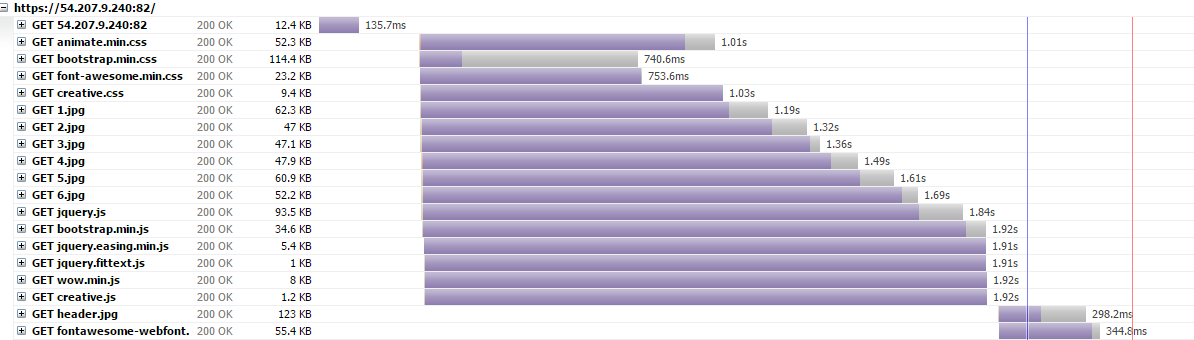
\includegraphics[width=1.0\textwidth]{./04-figuras/cascatas/template_http2}
\end{figure}
